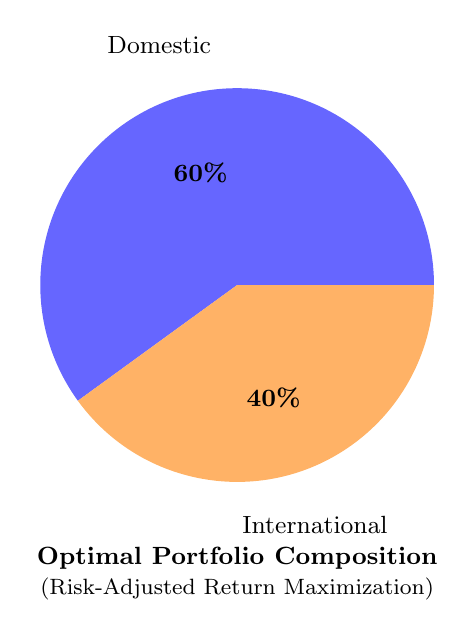
\begin{tikzpicture}
    % Simple pie chart using basic TikZ
    \def\radius{2.5}
    
    % Domestic sector (60% = 216 degrees)
    \fill[blue!60] (0,0) -- (0:\radius) arc (0:216:\radius) -- cycle;
    \node at (108:1.5) {\small\bfseries 60\%};
    \node at (108:3.2) {\small Domestic};
    
    % International sector (40% = 144 degrees)
    \fill[orange!60] (0,0) -- (216:\radius) arc (216:360:\radius) -- cycle;
    \node at (288:1.5) {\small\bfseries 40\%};
    \node at (288:3.2) {\small International};
    
    \node[below, font=\small\bfseries] at (0,-3.2) {Optimal Portfolio Composition};
    \node[below, font=\footnotesize] at (0,-3.6) {(Risk-Adjusted Return Maximization)};
\end{tikzpicture}
